\documentclass[tikz,border=4pt]{standalone}
\usepackage{amsmath,amssymb}
\usetikzlibrary{arrows.meta,calc,decorations.pathreplacing}
\definecolor{cA}{HTML}{924800}
\definecolor{cB}{HTML}{2F7FC8}
\definecolor{cC}{HTML}{39994B}
\tikzset{
  pt/.style={circle,fill=black,inner sep=0pt,minimum size=4pt},
  disp/.style={-{Stealth[length=2.6mm,width=2mm]},line width=0.9pt,shorten <=2.5pt,shorten >=2.5pt},
  lab/.style={font=\small,sloped,text=black},
  brc/.style={decorate,decoration={brace,amplitude=5pt,raise=3pt},line width=0.6pt},
}
\begin{document}
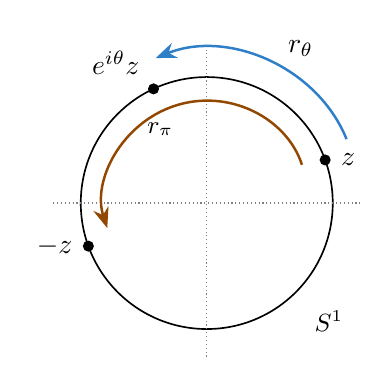
\begin{tikzpicture}
  \draw[line width=0.6pt] (0,0) circle (1.6);
  \draw[gray,densely dotted] (-1.95,0) -- (1.95,0); \draw[gray,densely dotted] (0,-1.95) -- (0,1.95);
  \coordinate (z) at (20:1.6); \coordinate (rz) at (115:1.6); \coordinate (mz) at (200:1.6);
  \draw[disp,cB] (22:1.95) arc[start angle=22,end angle=112,radius=1.95] node[pos=0.45,above right,text=black]{$r_\theta$};
  \draw[disp,cA] (18:1.3) arc[start angle=18,end angle=198,radius=1.3] node[pos=0.55,below,text=black,font=\small]{$r_\pi$};
  \node[pt,label=right:$z$] at (z) {};
  \node[pt,label=above left:$e^{i\theta}z$] at (rz) {};
  \node[pt,label=left:$-z$] at (mz) {};
  \node[font=\small] at (1.55,-1.5) {$S^1$};
\end{tikzpicture}
\end{document}
